\subsection{Decade Counter through Flip Flops}
%	
The 7474 IC has two D flip flops.  The D pins denote the input and the Q pins denote the output. CLK denotes the clock input.
\begin{problem}
Connect the 0-3 pins of the Pi to the Q pins of the two 7474 ICs. Use the 0-3 pins as Pi input.
\end{problem}
%
\begin{figure}[!ht]
\begin{center}
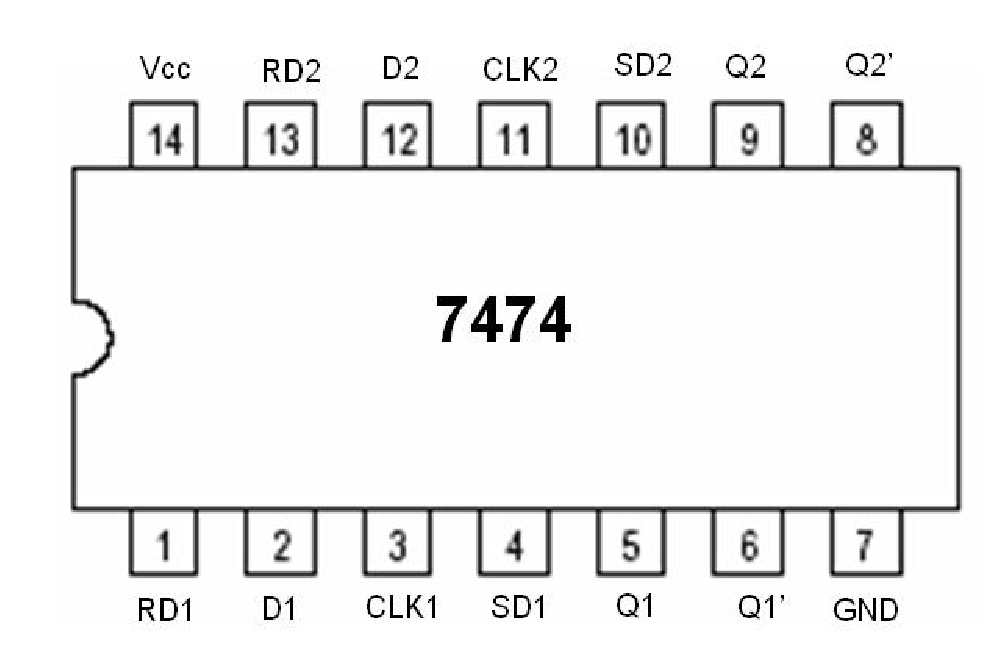
\includegraphics[width=\columnwidth]{./chapter4/figs/7474IC}
\end{center}
\captionof{figure}{Flip flop }
\label{fig_4_1}	
\end{figure}
%
\begin{problem}
Connect the Q pins to IC 7447 Decoder as input pins.  Connect the 7447 IC to the seven segment display.
\end{problem}
\begin{problem}
Connect the 11-14 pins of the Pi to the D input pins of two 7474 ICs. Use the 11-14 pins as Pi output.
\end{problem}
\begin{problem}
Connect pin 10 of the Pi to the CLK inputs of both the 7474 ICs.
\end{problem}
\begin{problem}
Using the logic for the counting decoder in the Pi software, implement the decade counter.
\end{problem}
%\begin{problem}
%Using the 0-3 pins as input and 11-14 pins as output, write a program to implement the logic functions in Problem \ref{seq_decoder} and execute the program.  Comment.
%\end{problem}


%\begin{problem}
%Draw the state transition diagram for the decade counter.  Number the states from 0-9
%\end{problem}
%\begin{problem}
%Draw the state transition table that has present and next state values in binary.
%\end{problem}

